\begin{figure*}[t]
	\centering
	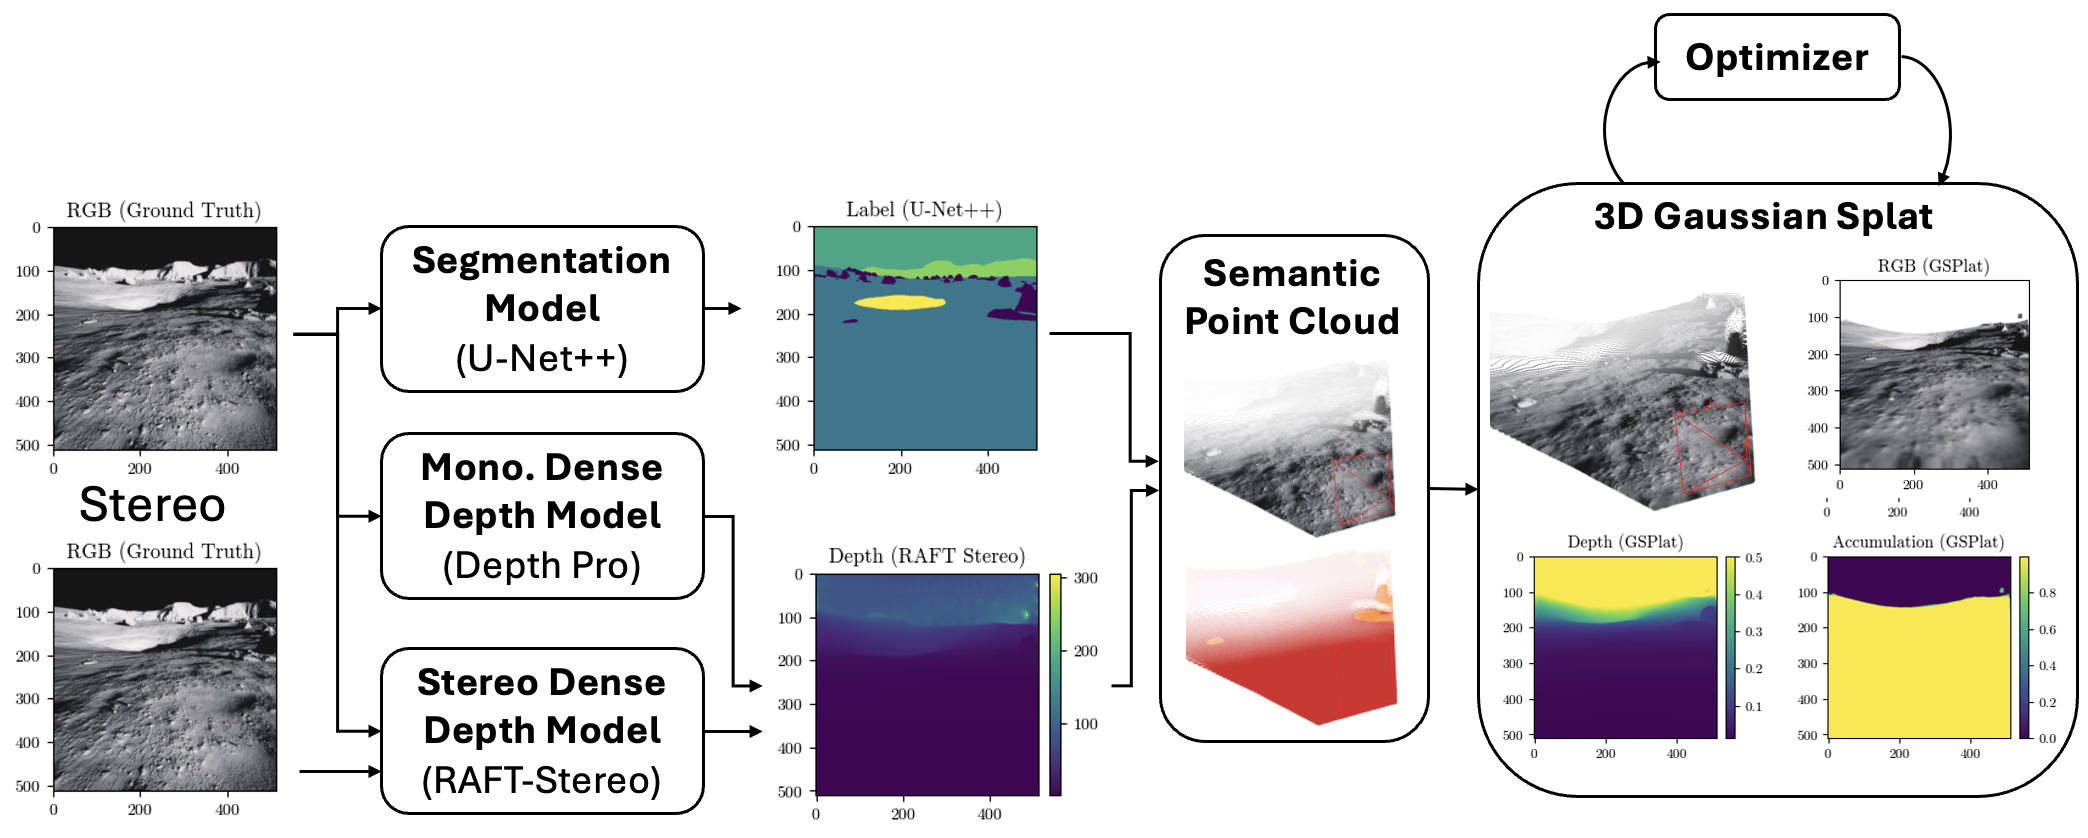
\includegraphics[width=0.75\linewidth]{diagram.png}
	\caption{\bfseries Diagram of the proposed method.}
	\label{fig:3dgs_diagram}
\end{figure*}

\section{Methodology}
Our primary contribution is a real-time pipeline for the incremental, semantic 3D reconstruction of the lunar surface using a 3D Gaussian Splatting (3DGS) representation. The framework is designed as the mapping component of a SLAM system, processing sensor data to build and continuously optimize a semantic 3DGS map. The architecture is composed of three principal stages: a perception frontend, an incremental mapping backend, and a keyframe-based optimization engine.

\subsection{Perception and Pose Frontend}
The frontend processes raw sensor data into a structured format. We assume that rover pose estimates are continuously available from an external tracking system, such as visual-inertial odometry; the development of this tracking component is outside the scope of this work. For each incoming camera frame, the frontend computes a dense depth map using either traditional stereo algorithms or monocular depth estimation networks, demonstrating modular support for various sensor configurations. Concurrently, a semantic segmentation network classifies each pixel into relevant lunar categories (e.g., regolith, rock), providing critical context. Pixels classified as sky are explicitly masked to prevent the erroneous creation of 3D points.

\begin{figure}[t]
	\centering
	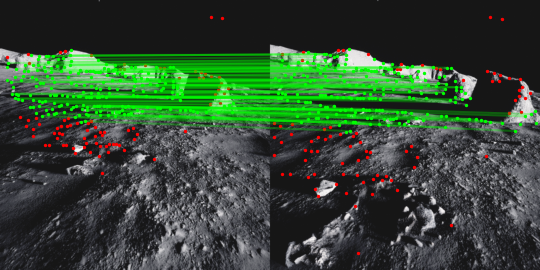
\includegraphics[width=\linewidth]{figures/matches.png}
	\caption{\bfseries Matches between consecutive frames used for monocular depth estimation scaling.}
	\label{fig:matches}
\end{figure}
For monocular depth estimation models, we employ a scaling strategy using triangulated points from matched features between consecutive frames. We detect and match keypoints using SuperPoint~\cite{detone_superpoint_2018} and SuperGlue~\cite{sarlin_superglue_2020}, as shown in \cref{fig:matches}, then triangulate these points to obtain metric depth estimates. We use these triangulated depths to scale the output of the monocular models. To ensure robust scaling, we apply depth masking to filter out unreliable matches and use random sample consensus (RANSAC) to remove outliers from the triangulated points. Specifically, we solve for the scale parameter $\theta$ and offset $\gamma$ by minimizing:
\begin{equation}
	\min_{\theta,\gamma} \sum_{p \in M_{\text{valid}}} \|\theta \hat{D}(p) + \gamma - D(p)\|_2^2,
\end{equation}
where $\hat{D}$ represents the estimated depth from the monocular model, $D$ is the ground truth depth from triangulation, and $M_{\text{valid}}$ is the mask of valid depth points after filtering.

\subsection{Incremental Mapping}
The backend receives the processed frames from the frontend and is responsible for incrementally building the global 3D map. For each new frame, the estimated pose, dense depth map, and semantic labels are fused to generate a registered, per-frame 3D semantic point cloud. This step transforms the 2D perception outputs into a 3D context where every point is associated with a color and a semantic class. This point cloud is then used to add new primitives to the global 3DGS model.
Each new Gaussian's size is set proportional to the average distance to its nearest neighbors, ensuring adaptive coverage based on local point density.
To maintain real-time performance and prevent unbounded map growth over long trajectories, a voxel-based filtering strategy is employed. Only 3D points that fall into previously unobserved regions of space are used to initialize new Gaussians in order to maintain real-time performance and prevent unbounded map growth. A key aspect of our system is that each new Gaussian is initialized with the semantic label from its corresponding point.

\subsection{Optimization Backend}
The optimization engine runs as a background process, continuously refining all Gaussian parameters and camera poses to improve global consistency.

\subsubsection{Keyframe-Based Asynchronous Optimization}
The system maintains a keyframe buffer that acts as a long-term memory, storing a history of processed frames. This is essential for preventing catastrophic forgetting, as the optimizer can periodically sample batches of past views to enforce global consistency. The optimization schedule is decoupled from a continuous step counter, allowing refinement to be triggered based on elapsed training intervals. This accommodates the asynchronous and intermittent execution of the optimization thread, making practical use of idle compute time during rover operations. While the Gaussian parameters are the primary target of optimization, the framework could be extended to refine camera poses as well; however, this is considered outside the scope of the current work.

\subsubsection{Densification Strategy}
To manage the set of Gaussians, we modify the standard 3DGS densification strategy. The data structure for each Gaussian is augmented to include a semantic class identifier. The periodic, global reset of Gaussian opacities is removed; this is critical for long-term mapping as our optimization prioritizes recent keyframes, and a global reset could cause stable, older portions of the map to be incorrectly pruned, leading to catastrophic forgetting. Furthermore, our implementation omits the standard splitting and cloning operations. Since the backend incrementally adds geometry from dense depth maps with each new keyframe, the large, under-reconstructed regions that typically necessitate splitting are less prevalent. Instead, we manage map complexity by pruning Gaussians that are inconsistent with a known prior DEM model.

\subsubsection{Loss Function}
The optimization process minimizes a total loss function, $\mathcal{L}_{\text{total}}$, which extends the standard 3DGS objective ($\mathcal{L}_{\text{recon}} + \mathcal{L}_{\text{scale}}$). The unique characteristics of lunar environments—namely high-contrast lighting and deep, hard-edged shadows with no atmospheric scattering—make relying on a simple background color insufficient. A deep shadow on the regolith can be photometrically indistinguishable from the black sky, providing ambiguous signals to the optimizer. To address this, we introduce explicit geometric and semantic supervision through additional loss components that use masks derived from sensor data.

These losses are applied selectively using two masks. The surface mask, $M_{\text{surface}}$, identifies pixels corresponding to valid geometry. A pixel is included in this mask only if it is not classified as sky, its estimated depth value is finite, and, very importantly, it is within a pre-specified depth range for optimization.
In this sense, a pixel that corresponds to a rock that is far from the current camera pose is not included in the surface mask.
The empty space mask, $M_{\text{empty}}$, identifies pixels known to contain no geometry and is primarily composed of pixels identified as sky.

Our additional loss components are:
\begin{itemize}
	\item \textbf{Supervised Depth Loss}: To leverage the dense depth maps from our perception frontend, we add a supervised depth loss, $\mathcal{L}_{\text{depth}}$. This term enforces geometric accuracy by penalizing the L1 difference between the rendered depth, $\hat{D}$, and the input depth map, $D$, only on the $M_{\text{surface}}$ mask:
	      \begin{equation}
		      \mathcal{L}_{\text{depth}} = \frac{1}{|M_{\text{surface}}|} \sum_{p \in M_{\text{surface}}} \frac{|D(p) - \hat{D}(p)|}{\max_{q \in M_{\text{surface}}} D(q)}
	      \end{equation}

	\item \textbf{Volumetric Regularization Losses}: To regularize the density distribution and remove artifacts, we use two losses based on the rendered alpha accumulation, $\hat{\alpha}$. An \textit{empty loss}, $\mathcal{L}_{\text{empty}}$, penalizes density in regions defined by $M_{\text{empty}}$. A complementary \textit{full loss}, $\mathcal{L}_{\text{surface}}$, encourages surfaces within $M_{\text{surface}}$ to be opaque:
	      \begin{align}
		      \mathcal{L}_{\text{empty}}   & = \frac{1}{|M_{\text{empty}}|} \sum_{p \in M_{\text{empty}}} \hat{\alpha}(p)           \\
		      \mathcal{L}_{\text{surface}} & = \frac{1}{|M_{\text{surface}}|} \sum_{p \in M_{\text{surface}}} (1 - \hat{\alpha}(p))
	      \end{align}
\end{itemize}

The final objective function is a weighted summation of the baseline and our new components:
\begin{align}
	\mathcal{L}_{\text{total}} =\  & \mathcal{L}_{\text{recon}} + \lambda_{\text{scale}}\mathcal{L}_{\text{scale}} + \lambda_{\text{depth}}\mathcal{L}_{\text{depth}} \notag \\
	                               & + \lambda_{\text{empty}}\mathcal{L}_{\text{empty}} + \lambda_{\text{surface}}\mathcal{L}_{\text{surface}}
\end{align}
where the $\lambda$ terms are the corresponding weighting coefficients.